\chapter{CFR-D and Decomposition}
\label{ch:cfr-d}
\epigraphLong{
  Everything that comes together falls apart.
  Everything.
  The chair I'm sitting on.
  It was built, and so it will fall apart.
  I'm gonna fall apart, probably before this chair.
  And you’re gonna fall apart.
  The cells and organs and systems that make you you--they came together, grew together, and so must fall apart.
  The Buddha knew one thing science didn't prove for millennia after his death:
  Entropy increases.
  Things fall apart.
}{John Green, \emph{Looking for Alaska}}
\vskip -2em
\note{
  This chapter summarizes the approach, methods and results of~the authors~\cite{BurchJohansonBowling2014}.
}

\section{Motivation and Overview}
The work of~(\cite{BurchJohansonBowling2014}) describes a~pioneering technique how to \emph{decompose} subgames of~imperfect-information games and solve them independently, while preserving the optimality of~the full-game solution.
Many benefits of~subgame re-solving are inherited from perfect-information games:
\begin{itemize}
  \item Run-time information (e.g., endgame actually reached during a~real play) can be exploited in a~smarter way.
  \item Memory and disk limitations (either at~run-time or while solving a~game) can be overcome by a~time/space trade-off.
  \item A~\acrlong{ne} for a~game larger than available storage may be computed.
  \item If we only need to work with one subgame at a~time, then significantly less storage is required.
  \item It is not obligatory to store the complete strategy, which might be too large to store.
    Instead, subgame strategies may be re-computed on~demand, when needed.
\end{itemize}

As for re-solving subgames in~the imperfect-information setting, all previous algorithms were limited to rather small domains, with the complete strategy that can fit in~available space.
As a~consequence, several appealing games still resist to be solved, despite the intensive effort put in~their research.
\note{
  This used to be the case for the two-player \acrshort{lhe}, until the~recent, highly-celebrated breakthrough by~the same research group (\cite{Bowling2015heads}).
}

\section{Gadget Game}
\epigraphLong{
  Dreams about the future are always filled with gadgets.
}{Neil deGrasse Tyson}
\vskip -2em
\note{
  We will distinguish the states, strategies, utilities, etc. and their translations to the gadget game by~adding a~tilde to corresponding notations.

  From now on for the rest of~the thesis, we will be refining the strategy for player~$1$ in a~two-player zero-sum game with the perfect recall.
}

Again, we start by~creating a~fine-grained abstraction for the subgame.
The original strategy for the subgame (from the coarse abstraction) is then translated into the fine-grained abstraction as $\sigma_1^S$.
The translated strategy is now used to compute $CBV_2 ^{\sigma_1^S} (I)$ for every information set~$I$ at~the root of~the subgame.
These values will be useful for the gadget construction to~guarantee the safety of~the resulting strategy.
See Figure~\ref{fig:re-solving-gadget} for a~sketch of~the construction.

\begin{figure}[H]
  \centering
  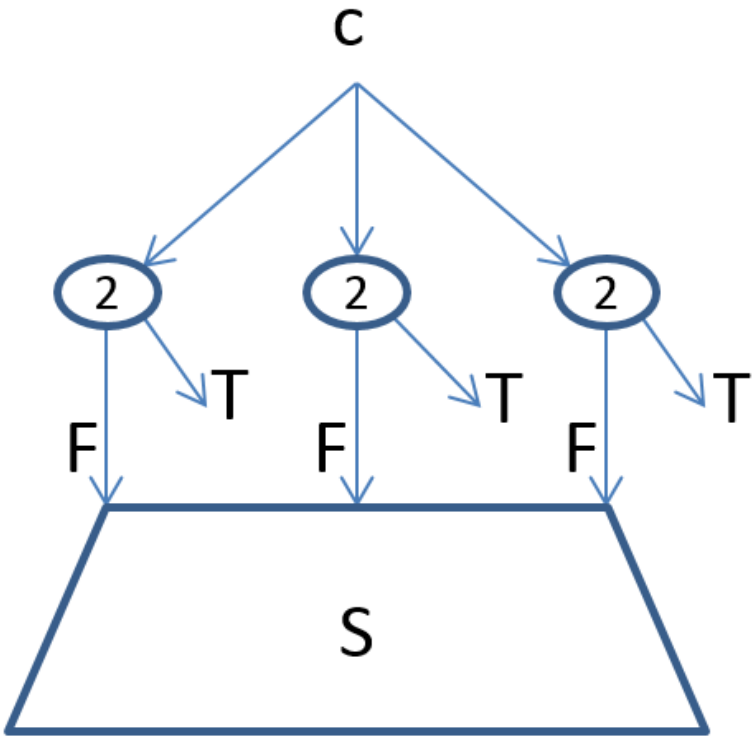
\includegraphics[width=.25\textwidth]{../img/re-solving-game-gadget.png}
  \def\captionTitle{A~gadget game for re-solving subgames}
  \caption[\captionTitle]{
    \captionTitle.
    The opponent chooses in~every state prior to the endgame either to (F)ollow the action into the endgame, or to (T)erminate.
    His utility after the (T)erminal action is set to his counterfactual best response in that state.
  }
  \label{fig:re-solving-gadget}
\end{figure}

To construct the gadget, we add one chance node at~the root of~the game, followed by additional nodes for player~$2$:
one for every state at~the root of the subgame.
At~each of~these nodes, $2$ may either accept the corresponding \acrshort{cbv} calculated earlier, or play the subgame (to get to the corresponding state at~the root of~the subgame).

The chance player distributes the player~$2$ into these states using the (normalized) $\pi^\sigma_{-2}$ (how likely is the state given that $2$ plays to reach it).
Since the game is zero-sum, this forces player~$1$ to play the subgame well enough, so that the opponent's value is no greater than the original CBV.
Acting like that, $1$'s overall game utility will not deteriorate:

\begin{thm}[\cite{BurchJohansonBowling2014}, Theorem~1]
  \label{thm:cf-val-and-utility}
  Given a~strategy $\sigma_1$, a subgame $S$, and a~re-solved subgame strategy $\sigma_1^S$, let $\sigma_1' = \sigma_{1, [S \leftarrow \sigma_1^S]}$ be the combination of $\sigma_1$ and $\sigma_1^S$.
  If $CBV_2^{\sigma'}(I) \leq  CBV_2^{\sigma}(I)$ for all information sets~$I\in\I_2^{R(S)}$, then $u_2(\sigma_1', \textrm{CBR}(\sigma_1')) \leq  u_2(\sigma_1, \textrm{CBR}(\sigma_1))$.
\end{thm}
\begin{proof}
  Consult the appendix of~(\cite{BurchJohansonBowling2014}).
\end{proof}

\section{Equivalent Linear Program}
This time, the presented \acrshort{lp} is not a~straightforward sequential-form representation of~the gadget construction.
Although such a~representation would be possible, it would not help to provide a~desirable insight.
Instead, we formulate an~\acrshort{lp} that solves the same game (for player~$1$) while demonstrating the underlying properties of~the re-solving approach:
\begin{equation}
  \label{lp:cfr-d}
  \begin{split}
    \max_{v, x}\ &0 \\
    \color{red}
      v_I - m &
    \color{red}
      \ge CBV_2^{\sigma_1}(I), \quad I \in \I_2^{R(S)}\\ 
    Ex &= e \\
    F^\top v - A_{\color{red}2}^\top x &\le \vect{0} \\
    x &\ge \vect{0},
  \end{split}
\end{equation}
where $\I_2^{R(S)}$ denotes the root information sets and $CBV_2^\sigma(I)$ is $2$'s original \acrlong{cbv} in~the information set~$I$.

The sequence payoff matrices $A_2$ and $A$ (from (\ref{lp:endgame-solving})) are slightly different, to reflect different strategies of~the chance player in the gadget for endgame solving (Figure~\ref{fig:endgame-solving-gadget}) and the gadget for re-solving subgames (Figure~\ref{fig:re-solving-gadget}).

The formulation uses the following fact:
any strategy, where the opponent's \acrshort{cbv} is not greater than the original one, is a~solution to the game.
This follows from the construction of~the gadget for re-solving games.

It is worth remarking three important points:
\begin{enumerate}[(1)]
  \item (\ref{lp:cfr-d}) is not optimizing any value ($0$ is a~constant).
    Instead, the \acrshort{lp} looks for a~feasible solution.
    Though theoretically equivalent, in this case it is semantically different for the strategy.
  \item The original, unrefined strategy is a~feasible solution to (\ref{lp:cfr-d}).
  \item Points (1) and (2) might suggest the strategy may not improve.
    Empirical evaluations show otherwise however:
    using a~\acrshort{cfr} algorithm to solve the gadget game, the performance of~the refined strategy improves over the original (\cite{BurchJohansonBowling2014}).
    Our experiments further confirm this (Section~\ref{sec:max-margin-experiments}).
\end{enumerate}

\section{Discussion}
The innovative aspect of~(\cite{BurchJohansonBowling2014}) consists of~two main contributions:
\begin{itemize}[(i)]
  \item A~technique to re-solve imperfect-information subgames, which is guaranteed not to increase sub-optimality of~the resulting full-game strategy.
    Owing to summary information about a~subgame strategy (namely the \acrlong{cbv}s), the newly generated strategy is no more exploitable than the original one.

  \item A~new off-line solving algorithm called \emph{\acrfull{cfr-d}}, capable of~computing an~error-bounded \acrshort{ne} approximation.
    \acrshort{cfr-d} achieves this by decomposing and independently analyzing subgames.

    By~sacrificing computation time, the decomposition allows for \emph{sub-linear space costs}.
    For instance, two-player \acrshort{lhe} with \acrshort{cfr-d} can be solved in less than 16 GB, rather than~more than 200 TB of~disk space!
\end{itemize}
